\documentclass[twocolumn]{article}

\usepackage[utf8]{inputenc}
\usepackage[T1]{fontenc}
\usepackage{apalike}
\usepackage{graphicx}
\usepackage{amsmath}
\usepackage{amsfonts}
\usepackage{booktabs}
\usepackage[margin=1in]{geometry}
\usepackage{mathrsfs}
\usepackage[english]{babel}
\DeclareMathOperator*{\argmin}{argmin}
\DeclareMathOperator*{\argmax}{argmax}
\usepackage{csquotes}
\usepackage{siunitx}
\usepackage{bookmark}
\usepackage[style=authoryear,natbib=true,backend=bibtex]{biblatex}
\usepackage[compact]{titlesec}
\setlength{\pdfpagewidth}{8.5in}
\setlength{\pdfpageheight}{11in}
\setcounter{secnumdepth}{0}
\renewenvironment{abstract}{\centerline{\bf
Abstract}\vspace{0.8ex}\begin{quote}}{\par\end{quote}\vskip 1ex}
\bibliography{bibliography.bib}
\setlength{\parindent}{6ex}
\usepackage{etoolbox}
\usepackage{hyperref}
\makeatletter
\patchcmd\@combinedblfloats{\box\@outputbox}{\unvbox\@outputbox}{}{\errmessage{\noexpand patch failed}}
\makeatother


\title{\textbf{Deep Reinforcement Learning in Natural Language Processing: A Global Review}}
\author{\textbf{Mathieu Godbout}\\
\textit{mathieu.godbout.3@ulaval.ca}\date{}
}


\begin{document}

\maketitle

\begin{abstract}
\begin{quote}
Deep supervised learning offers great promise on the variety of Natural Language Processing tasks. Such approaches are however faced with performance limitations, possibly caused by employing different scoring metrics at train and test time. Such discrepancy is caused by the differentiability requirement for losses used in backpropagation training and the greater significance of non-differentiable metrics like BLEU and ROUGE for model evaluation. In order to provide a solution to this problem and subsequently achieve greater performance, Reinforcement Learning (RL) has been applied on numerous NLP tasks. This paper provides a global review of RL approaches in NLP, emphasizing on the different steps required to build a RL model on NLP tasks as well their motivation.
\end{quote}
\end{abstract}

\section{Introduction} 
Reinforcement Learning\footnote{We will use the terms Reinforcement Learning and Deep Reinforcement Learning interchangeably in this article, given the large majority of recently published papers about Reinforcement Learning implementing some sort of Deep Reinforcement Learning.} (DRL) is a machine learning technique that sees a given task as an environment in which an agent evolves by trying to select the maximum rewarding possible action for its current state. After its successful applications to Atari Games \citep{mnih2015humanlevel} and the Go game \citep{Go}, DRL has been a subject of rapidly growing interest. This interest spread to the field of Natural Language Processing (NLP), sparkled by the promising results of the technique as well as by the relatively easy reformulation of many NLP tasks as RL problems. Behind the stated great successes of reinforcement learning of known hard problems lie two main characteristics that distinguish the technique from other classical deep supervised learning approaches. 

First of all, since the RL formulation of a problem only requires some sort of real-valued reward for given actions, RL networks are no longer needed to fit a differentiable scoring metric \citep{ranzatoCAZ15}, as in the classical supervised framework. Hence, as most NLP testing metrics are discrete and non-differentiable, like \textit{BLEU} \citep{BLEU} and \textit{ROUGE} \citep{ROUGE} scores, RL can be used to go around what we will call test and train metrics discrepancy, where a model is trained to maximize a given metric but is then tested on another, with which it does not necessarily have solid correlation. 

The second very interesting characteristic of reinforcement learning is its generalization aptitude (\cite{kaelbling1996reinforcement}; \cite{sutton-generalization-rl}). When tuned carefully, reinforcement learning algorithms have been empirically shown to be less prone to overfitting, at the usual cost of slower convergence. This essentially means that, when applied to natural language tasks, RL should be able to better approximate a global maximum of the learned task, especially in languages where available data is massive, such as English.

Perhaps quite promising, reinforcement learning is not without any flaw. An important one of which is found in its convergence inefficiency on large state or action spaces. In the technique, the trained agent has to explore an environment and the possible actions made in each state of the environment. Therefore, the learning task complexity grows in correspondence to the formulation model's state and action spaces' complexity. While many NLP tasks can be easily reformulated as RL problems, the new formulation almost always has immense state and/or action space complexity. This is therefore a core problem that most suggested approaches try to address one way or another when applying reinforcement learning to NLP.

The current paper aims to provide a global review of recent usages of reinforcement learning in NLP. Building on a basic knowledge of the most prominent NLP tasks, we will focus more on how can RL be applied to them from the point of view of NLP researchers. Furthermore, emphasis will be put on the different overall learning strategy rather than on various implementation details, aiming to provide a wider yet comprehensive review over the variety of tasks in Natural Language Processing.

This paper begins by providing a more technical overview of the reinforcement learning technique, exploring its structure, algorithms, as well as its possible drawbacks. A brief explanation of the reviewed NLP tasks and their typical formulation then follows. After will be presented the different ways RL has been applied to natural language processing, particularly exploring the different challenges it tries to overcome. 

\section{Reinforcement Learning}

The main idea behind RL is to consider a problem into a sequential decision making process, typically a Markov Decision Process, consisting of an agent evolving in an environment $\Sigma $ taking actions \textit{$a_t$} at discrete time steps \textit{t} \citep{sutton2018reinforcement}. After the agent picks action \textit{$a_t$} in environment state \textit{$s_t$}, the environment returns the reward \textit{$r_{t+1}$} and next state \textit{$s_{t+1}$}. This overall process is shown in figure~\ref{fig:rl}. For every time step, the agent picks an action $a_t \in \mathcal{A}$, where $\mathcal{A}$ is the set of all available actions. To do so, the agent follows a policy $\pi(a_t|s_t)$, effectively matching a state to the expected best action. The best action is judged upon the expected discounted reward collected by an agent following policy $\pi$, namely
$R_t^{\pi} = \sum_{\tau=t}^\infty \gamma^{\tau - t}r_{\tau}$, where $\gamma \in [0, 1]$ is discount factor that balances the importance of immediate and future rewards. At last, the RL paradigm can be summed up to learning the optimal policy $\pi^*$, where

\begin{equation*}
\pi^* = \argmax_{\pi} \> R_t^{\pi} = \sum_{\tau=t}^\infty \gamma^{\tau - t}r_{\tau}
\label{eq:pi_star}
\end{equation*}

\begin{figure}[]
\centering
\vspace*{-0.15in}
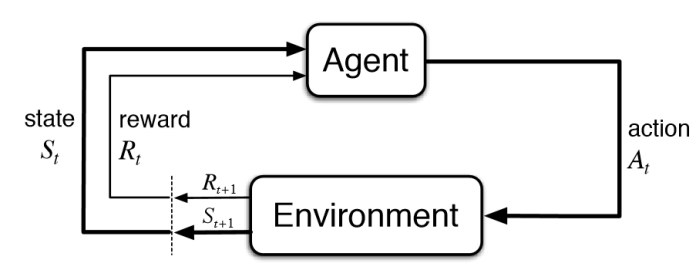
\includegraphics[scale=0.55]{reinforcement-learning-fig1-700.jpg}
\vspace*{-0.3in}
\caption{Illustration of the discrete relation between an RL agent and the environment it evolves in.}
\label{fig:rl}
\end{figure}


Hence, most of the research in RL is focused around different optimization tricks aimed towards finding $\pi^*$ or another satisfying policy for a given environment. In order to address this, for an agent following policy $\pi$, functions defining the expected value of a state-action pair $Q(s_t, a_t)$ and of a state $V(s_t)$ have been introduced, as follows:

\[
\begin{array}{l}
Q_{\pi}(s_t,a_t) = \mathbb{E}[R_t|s_t, a_t]  \\
V_{\pi}(s_t) = \mathbb{E}[Q_{\pi}(s_t,\pi(s_t))]
\end{array}
\]

\noindent From the above equations, a greedy deterministic policy could simply be to choose $a_t = \argmax_a Q(s_t,a)$. 

One of the key problems with the above approach is that it requires great computational effort to obtain a single value of the $Q$ or the $V$ functions. A possible way to go around this problem would be to simply store the values of either desired function in a table, only requiring an initial setup. However, in fields where the state and action space are very large - such as NLP, since the system is required to evaluate every single possible (state, action) pair, such an approach can hardly be considered, due to memory and time limitations. 

Recently, deep neural networks have been successfully proposed as a solution by trying to provide accurate estimates of the value functions \citep{DBLP:journals/corr/Li17b}. Although the proposed approaches vary widely, they are all built around the same high-level algorithm. They all collect true values data, per example (state, action) pairs linked to their correct $Q$-value, and attempt to generalize this data to obtain as good as an approximation possible for unseen pairs. Recent approaches like Deep Q-Network \citep{mnih2015humanlevel} and AlphaGo \citep{Go} have managed to stabilize the learning and achieve outstanding results.

 Another way to go around the inherent difficulties linked with large state-action spaces is a family of algorithms called REINFORCE \citep{Williams:1992:SSG:139611.139614}. Let us consider a policy network $\pi_\theta$, where $\theta$ represents the policy network's learnable parameters. A REINFORCE algorithm will directly update $\theta$, given an action-pair and the corresponding observed reward. These methods therefore essentially bypassing the need for the above mentioned function approximation techniques. The whole idea is to update $\theta$ according to the following rule
 
 \begin{equation*}
\Delta \theta = \nabla_{\theta} \log \pi_{\theta} (a_t|s_t)v_t,
 \end{equation*}

\noindent where $v_t$ is a sample of the value function at time $t$ collected from experience. 

The approaches presented above all aim to obtain convergence to a satisfying agent policy $\pi^*$. However, since the policy training is solely focused around maximizing an expected reward function, the reward function has to be as reflective as possible of the desired model's comportment. This is why reward function fine-tuning is an important part of any RL model. What actually makes reward function design an interesting problem is that the reward function can be, by definition, any function that takes a state $s_t$ and returns a corresponding real-valued reward $r_t$. This eliminates the need for differentiability, which is key to any backpropagation approach in classical supervised learning. Furthermore, this means that the reward function can be very complex or not continuous, essentially providing RL researchers with immense freedom in this domain. For example, one such interesting approach to reward optimization is to deduct a baseline reward $b_t$ from the perceived reward $r_t$, where $b_t$ could be the agent's maximum perceived reward in the visited state, allowing a policy to update on its own past performance.

\section{Natural Language Processing}

Natural Language Processing can be thought of as the group of all problems centered around human language where the desired solution has to be automatic. Such problems are numerous and vary widely, going from information extraction to sentence generation and others. Since the scope of this paper is to explore the usages of RL in NLP, we will however settle our attention on only some of the NLP tasks for which RL usages have been the most interesting from our point of view. Before diving into task explanation, we first describe common ground training algorithms as well as testing metrics.

First of all, NLP data is usually referred to as a \textit{corpus} that consists of numerous sentences or texts and the corresponding expected output of an automatic program trained for the task. For example, in machine translation, the corpus could simply be made of translated sentences from one source language to another target language. Due to the usual availability of large corpus, deep learning techniques have been applied with a lot of success to the field. Also because of the intrinsic recurrence in language, most state-of-the-art performing approaches on NLP tasks are currently centered around recurrent neural networks (RNNs) \citep{elman}. The usual training protocol of any supervised learning technique is focused around the minimization of cross-entropy loss, modeled to each given task.

Albeit interesting for training, cross-entropy comparison to a target hardly reflects the complexity of the human language and is therefore rarely used to evaluate the final performance of a given model. To provide with automatic evaluation metrics that capture more of the intrinsic richness of language, two main metrics have been proposed: BLEU \citep{BLEU} and ROUGE \citep{ROUGE}. BLEU essentially evaluates subsentences overlapping \textbf{precision} between a produced sentence and one or more target sentences, paired with a brevity penalty, for encouraging rich sentences. ROUGE on the other side of things focuses more on the subsentences \textbf{recall} between a produced sentence and a target sentence. Both of those metrics are the most prominent in tasks explored in this paper, with each one being more naturally inclined to some tasks than others.

The first one of the presented tasks is known as \textbf{text classification}. In this task, the goal is to match an input text to a certain category inside a set possible categories set. For example, this could consist of being able to distinguish newspaper articles based on which section of the newspaper they appeared in (arts, sports, news, business, etc.). This task is pretty straight forward machine learning as in the targets are fixed and the evaluation metric can be as simple as simple accuracy.

Another important task of NLP is the called \textbf{information extraction}. In information extraction, a model is learned to retrieve some key components from a given text. For example, one such task could be articulated around the extraction of pertinent info (murderer, number of victims, etc.) given a homicide crime report. In this context, since the target output is a single word per search criteria, the training and evaluation metrics can both be based upon prediction accuracy.

One particularly hot topic in Natural Language Processing is everything that revolves around \textbf{text generation}. In this type of problem, a model is trained on trying to generate a sequence of words that will be coherent as a sentence in the desired context. Many tasks are centered around this key problem, per example, text summarization and machine translation. Such tasks cannot be correctly evaluated by simple accuracy due to the possibility of sentences essentially saying the same thing but differing vastly in word choices. This is why models trained for this problem are usually compared on whatever metric of BLEU or ROUGE best suits the specific task's target output. However, since those two metrics are both discrete and non-differentiable, they cannot be used at training time in any backpropagation approach. This is why the classical training procedure is still based on the cross-entropy loss, essentially creating what we called earlier the test and train metrics discrepancy.

The last NLP task we present is \textbf{question answering}. The usual data format on this task consists of a series of questions and their expected (words) answers. The best performing approaches are based on a multi-system approach, where one system is in charge of extracting important question features, another of finding pertinent information on the matter and the last has to predict a sentence from the relevant information retrieved. Although a bit more complex, this whole system's training is still centered around backpropagation techniques, trying to minimize the cross-entropy-loss of the model's predicted outcome. Once again, evaluation can be done on any accuracy-based score for question answering. 

\section{Reinforcement Learning in NLP}

Reinforcement learning in natural language processing has seen an immense grow in interest in terms of published papers in the last years. Excellent and more technical reviews of reinforcement learning in general \citep{DBLP:journals/corr/Li17b} as well as reinforcement learning in sequence to sequence models \citep{DBLP:journals/corr/abs-1805-09461} and machine translation \citep{DBLP:journals/corr/abs-1808-08866} can be found in the literature for an exhaustive view on the matter. This paper detaches itself from previous work by providing a more high-level overview of usages of RL in NLP. Specifically, we limit our exploration of the proposed approaches to the topics of problem formulation, reward design, training strategies and more advanced RL techniques applied to NLP.

\subsection{Problem formulation}

As stated earlier, many NLP tasks can be easily thought of in terms of a Markov Decision Process (MDP) and therefore provide a natural application field for reinforcement learning techniques. From a broader point of view, the different proposed MDP frameworks for the explored reinforcement learning tasks can be split in two distinct groups: agent learning and data augmentation.

\subsubsection{Agent learning}

When talking of \textbf{agent learning}, we mean to speak of any context in which an RL agent is seen as the only component of a learning model. Candidate tasks for this approach all have in common the sequence output format they wish to produce. The generation of a sequence of words as an iterative process in which the next word in a given sentence is based upon the already selected words. This quite naturally fits a MDP model, where possible actions are all vocabulary words and states are the preceding sequence of already chosen words. This RL formulation has been successfully applied in question answering \citep{DBLP:journals/corr/BuckBCGHGW17}, sentence simplification \citep{sentence_simplification} as well as text summarization, machine translation and image captioning \citep{ranzatoCAZ15}.

\citep{DBLP:journals/corr/Li17b} further built on this framework on the topic of dialogue generation. Their proposed MDP formulation differs by considering the action set to be all possible dialogue utterances - see sequences - and the state to be the concatenation of the last dialogue utterance of each one of the two conversational agents.

\subsubsection{Data augmentation}

On the other hand, \textbf{data augmentation} usages of RL in NLP use way more diverse MDPs, representing in what way the data is desired to be augmented for a given task. For example, \citep{DBLP:journals/corr/abs-1805-09927} applied RL to the problem of filtering noisy data in relation extraction. They propose a framework where actions are to either retain or filter a given sentence, using the given sentence and previously removed sentences as state. In a similar fashion, \citep{DBLP:active_learning} apply RL-based active learning to the task of part-of-speech tagging. Their action set is once again binary, to tag or not an input sentence, and their state is represented by the current sentence and previously selected sentences to be tagged.

\citep{learning-structured-representation-text-classification-via-reinforcement-learning} also present two quite interesting approaches to the text classification task. They argue that reformulation or filtering of input sentences would help a classifier achieve better results. They first introduce a filtering agent, who acts upon a given input sentence, with the action set of keeping or removing a word, while state representation is the whole sentence. The second agent they introduce is aimed at splitting an input sentence into smaller, highly coherent, subsentences. The action space is now to either add a word to the current running subsentence or to create a new subsentence at this point, while the state now also contains information on the current running subsentence.

\subsection{Reward design}

One of the principal contribution of reinforcement learning to NLP is centered around the flexibility of reward functions over typical supervised learning loss functions. Mainly because reward functions are free of the restriction of being differentiable, complex metrics such as BLEU and ROUGE can now be used during the whole training process instead of just as a performance scoring metric. Moreover, reward functions are also allowed to incorporate custom behaviour, such as the introduction of state-category specific metrics \citep{DBLP:journals/corr/Guo15b}. 

Furthermore, the flexibility given to reward functions has also led to domain-specific metrics being being introduced to lead to qualitatively better results. For example, \cite{D18-1353} teach an agent to generate poetry from a weighted sum of domain-specific metrics such as meaningfulness, fluency and coherence. A similar sum of domain-specific metrics was also applied on dialogue generation by \citep{DBLP:journals/corr/LiMRGGJ16}.

Let us also note the frequent usage of reward reshaping by the deduction of a basic reward $b_t$ from the perceived reward $r_t$. The basic reward being usually based on the mean of last perceived rewards or on a precedent best reward perceived at a given state, this trick basically reformulates the RL problem as a problem of self-optimization. The basic reward deduction technique has been shown to alleviate the problem of high variance in RL convergence \citep{drl-that-matters}.

Finally, another important part of reward design is the choice between immediate or delayed reward. In both presented approaches (agent learning and data augmentation), rewards are typically zero throughout all the decision process until the agent gets to a terminal state, either the end of a sequence or the end of a dataset.

\subsection{Training strategies}

From the above presentations, two main challenges arise surrounding the application of RL in NLP. First, while the presented agent learning MDPs consist of very basic, if any, modifications to classical approaches in their respective task, the simplicity of the reformulation comes at the cost of very large  action and state spaces. For example, given a vocabulary $V$, we would have action space $A \in \mathcal{O}(|V|)$ and state space $S \in \mathcal{O}(|V|^T)$, where $T$ is the fixed maximum sentence length. Second, in data augmentation MDPs, since rewards are typically only observed once the end of the dataset is reached and a single training epoch is really time consuming, convergence is typically hard to reach.

\subsubsection{Hot-start}

Both of these problems have the same consequence: they make the usual beginning random policy approach very inefficient and prone to divergence. It is with this in mind that \textit{hot-start} approaches have been proposed, where the agent policy is initialized to some parameters we know to be closer to a global reward function maximum. The proposed initialization is always based on the classical cross-entropy loss, known to be able to produce interesting results. One direct hot-start method could, for example, simply be to begin training with a reward function after a decent cross-entropy loss training. Interesting algorithms have also been proposed to progressively replace cross-entropy loss with the desired reward function.

The first of those algorithms is to use a new reward $R'$ that consists of the sum of the cross-entropy loss and target reward $R$ :

\begin{equation*}
R' = \lambda(t) \textit{CELoss} + (1-\lambda(t))R,
\end{equation*}

\noindent where $\lambda(t)$ is a scalar function that gradually decays from 1 to 0 as the number of epoch $t$ grows. 

\citep{ranzatoCAZ15} proposed another algorithm to provide \textit{hot-start} policy called MIXER. The MIXER approach varies the reward the agent perceives at every epoch from a pure cross-entropy loss to the pure target reward function. To do so, they propose to split training into epoch batches, that begin by only cross-entropy training epochs and gradually introduce RL training epochs in the batches. 

\subsubsection{Optimization algorithms}

As presented earlier in the section on Reinforcement Learning, optimization in order to retrieve an optimal policy $\pi^*$ can mainly be done through two approaches: value-based and policy-based techniques. The most popular implementation of value-based algorithms, namely Deep Q-Network \citep{mnih2015humanlevel}, has been applied in both the agent learning \citep{DBLP:journals/corr/Guo15b} and data augmentation (\cite{DBLP:journals/corr/NarasimhanYB16}, \cite{DBLP:active_learning}) frameworks. On the other hand, the most famous policy-based family of algorithms, REINFORCE \citep{Williams:1992:SSG:139611.139614}, has also seen use in both problem formulations (\cite{ranzatoCAZ15}, \cite{DBLP:journals/corr/BuckBCGHGW17}, \cite{learning-structured-representation-text-classification-via-reinforcement-learning}, \cite{Zeng2018LargeSR})\footnote{Note here that the given citations are only informal of the most pertinent implementations of the discussed optimization algorithms in their problem formulation group. Any other cited paper presenting a RL approach to NLP also settled to either policy-based or value-based algorithms.}.

No conclusive observation can be done on which one of the optimization algorithms is most pertinent to NLP tasks in light of published results. They have both been shown to have similar successes, but, to our knowledge, no research paper has explored the two algorithms' performance on the same task, making it hard to draw a fair comparison. Essentially, both suffer from the mentioned problem of large state and action spaces as well as the delayed reward issues, without any displaying clear convergence or computational advantages.

\subsection{Advanced techniques}

Although very interesting, the previously presented approaches all remained quite shallow in terms of RL techniques exploration, preferring the proven and more conservative techniques over the more advanced but challenging ones. Such advanced techniques have however been proposed recently, mainly in an attempt to improve performances. We present a few of the most prominent work in that matter.

A first very interesting RL advance is the combination of both policy gradient and value function optimization algorithms through a model called \textit{actor-critic} \citep{sutton2000policy}. In this model, a policy-based agent (the actor) is trained in pair with a value-based agent (the critic). Both models are paired in a way that the actor's perceived rewards are based upon the critic's output value, and vice-versa. This approach has mostly been used in the agent learning framework, to sequence generation topics like text summarization \citep{jurafksy} and machine translation (\cite{BahdanauBXGLPCB16}, \cite{decoding-value-networks}, \cite{jurafksy}). The introduction of actor-critic methods has helped the above approaches to surpass or obtain state-of-the-art performance on their respective tasks, mostly by accelerating the learning convergence.

Another problem posed by naive RL implementation in NLP tasks that has seen solution attempts is the delayed reward problem. In order to correct the situation, a potential-based approach \citep{Ng:1999:PIU:645528.657613} is the most famous way to proceed. In potential-based rewards, the attempt is to be able to assign an estimation of the potential delayed reward a state-action pair ($s_t$, $a_t$) will receive. In order to implement this technique to value-based agents, one could simply add a ($s_t$, $a_t$, $r_t$) tuple to the training set in which $r_t = \gamma^{T-t} r_T$, where $T$ is the time step of the perceived delayed reward, building from experience play. This approach is particularly fit for actor-critic approaches. Notably, \citep{20q-games} introduce a RewardNet neural network to get immediate rewards on the task of a question asking based game. They propose to have a neural network trained on the potential-based reward instances to provide generalizable immediate rewards to their policy-based agent. Adding to this, \citep{BahdanauBXGLPCB16} build upon this proposition by shaping the reward for a time step $t$ as the subtraction of the above mentioned $r_t$ and $r_{t-1}$, providing a more adapted reward to the iterative nature of sequence generation in the machine translation task.

\section{Conclusion}

In this paper, we provided a general overview of the recent advances
in applying Reinforcement Learning  (RL)  techniques on Natural Language Processing (NLP) tasks. NLP has a broad range of application fields, going from machine translation to text summarization. Even though the domain has seen many performance improvements after the introduction deep supervised learning models, traditional models in this field
usually suffer from various problems during model training,
such  as  inconsistency  between  the  training  objective  and
testing objectives. Recently, with advances
in  deep  reinforcement  learning,  researchers  offered  various  types  of  solutions  to  combine  the  RL  training  with task-specific training for alleviating the problems and challenges
they usually face.  In  this  paper,  we  summarized
some  of  the  most  important  works  that  tried  to  combine
these two different techniques by providing a decomposition of the different RL model design steps from a NLP perspective.

\printbibliography

\end{document}

